% Chapter Template

\chapter{Definición del problema}

\label{Chapter5} % Change X to a consecutive number; for referencing this chapter elsewhere, use \ref{ChapterX}

\section{\textit{The Nature Conservancy Fisheries Monitoring }}

En el océano Pacífico, donde se captura más del 60\% del atún del mundo, tienen
lugar prácticas de pesca irregular que amenazan a los ecosistemas marinos y a
la estabilidad de la pesca mundial. \textit{The Nature Conservancy} es una
asociación que trabaja con organizaciones locales y globales para preservar las
especies marinas de cara al futuro.

La principal idea para controlar la pesca y explotación de recursos marinos es
el uso de cámaras en barcos, que ayudan a monitorizar las actividades pesqueras
de estos. Aunque funciona muy bien como sistema de control, la cantidad de
datos e imágenes generadas hace que sea muy costoso de procesar manualmente.

\begin{figure}
  \centering
  \caption{Ejemplo de imágenes tomadas en barcos pesqueros para su posterior identificación}
\label{kaggle-banner}
  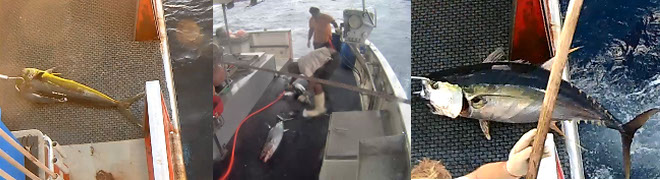
\includegraphics[width=\textwidth]{kaggle-competition-banner}
\end{figure}

La idea de este reto es desarrollar algoritmos que detecten y clasifiquen
automáticamente especies de atunes, tiburones y otras especies que estos barcos
pesqueros cazan. El que se pueda analizar rápida y automáticamente imágenes
como las de la figura \ref{kaggle-banner} permitirá asignar recursos de una
manera mucho más efectiva para el control de este tipo de actividades
\parencite{kaggle-page}.

\section{Definición del problema}

El problema consiste en clasificar cada una de las imágenes de un conjunto de
imágenes de barcos en una de las ocho categorías disponibles. Las imágenes
suelen mostrar la cubierta de un barco donde puede aparecer un pez. En base al
pez que aparezca hay que clasificarlo en una de las seis categorías mostradas
en la figura \ref{kaggle-fishes}.

\begin{figure}
  \centering
  \caption{Especies de peces a clasificar en el reto}
\label{kaggle-fishes}
  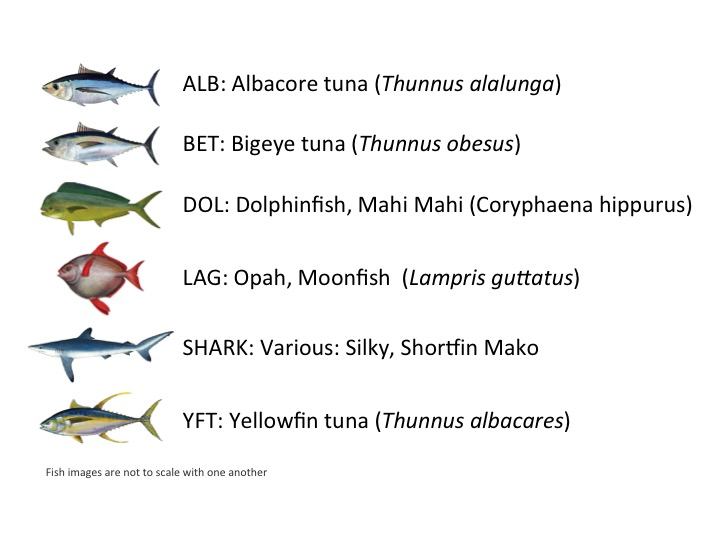
\includegraphics[width=\textwidth]{species-ref-key}
\end{figure}

En caso de que no aparezca ningún pez en la imagen, esta tendrá la categoría NOF (\textit{No Fish}). Y si aparece un pez en la imagen no perteneciente a ninguna de las categorías mencionadas, la categoría será OTHER.

En resumen, el conjunto de posibles categorías es:
\[
  categories =
  \left[ALB, BET, DOL, LAG, SHARK, YFT, OTHER, NOF]
\]

\subsection{Datos}

La competición proporciona tres ficheros con los que trabajar:

\begin{enumerate}
  \item{Conjunto de datos de entrenamiento: 3777 imágenes etiquetadas con una de las ocho categorías existentes.}
  \item{Conjunto de test y evaluación: 1000 imágenes sin etiquetar.}
  \item{Archivo de envío de prueba: Archivo CSV que muestra la estructura que debe tener el archivo con las soluciones}
\end{enumerate}

\subsection{Envío de la solución y evaluación}
\label{sec:envio-y-eval}

Para el envío de la solución hace falta clasificar las 1000 imágenes del conjunto de evaluación, indicando la probabilidad de que pertenezca a cada una de las ocho categorías diferentes. En el cuadro \ref{submission-sample} se muestra un ejemplo de algunas filas del archivo CSV a enviar.

\begin{table}[]
\centering
\caption{Ejemplo del archivo de envío}
\label{submission-sample}
\begin{tabular}{lllllllll}
image          & ALB   & BET   & DOL   & LAG    & NoF   & OTHER & SHARK  & YFT  \\
img\_00005.jpg & 0.455 & 0.052 & 0.030 & 0.0173 & 0.123 & 0.079 & 0.046 & 0.194\\
img\_00006.jpg & 0.455 & 0.052 & 0.030 & 0.0173 & 0.123 & 0.079 & 0.046 & 0.194\\
img\_00007.jpg & 0.455 & 0.052 & 0.030 & 0.0173 & 0.123 & 0.079 & 0.046 & 0.194\\
\end{tabular}
\end{table}

Los resultados enviados se evalúan mediante una función de pérdida logarítmica multiclase. Concretamente se usa la fórmula
\[
  logloss =
  - \frac{1}{N} \sum_{i=1}^N \sum_{j=1}^M y_{ij} \log \, p_{ij}
\]
 siendo N el número de imágenes en el conjunto de test, M el número de
 categorías, $y_{ij}$ 1 si la observación $i$ pertenece a la categoría $j$ y 0 si no
 pertenece y $p_{ij}$ la probabilidad predicha de que el elemento $i$ pertenezca
 a la categoría $j$.

 Cuanto menor sea el valor obtenido, mejor se habrá comportado el modelo sobre el conjunto de prueba.

\subsection{Tablas de clasificación y fases de la competición}

Cuando un participante envía una predicción, \textit{Kaggle} calcula la
puntuación de dicho envío sobre un subconjunto de ejemplos compuesto del 8 \%
del conjunto de test, mostrando la puntuación en una tabla de clasificación
pública. Se usa un subconjunto para evitar que los participantes puedan
aprovechar un sobreajuste a la hora de entrenar el modelo.

Antes de terminar la primera fase de la competición los participantes deberán subir a \textit{Kaggle} el modelo utilizado y seleccionar las dos predicciones que quieren usar para la puntuación con el conjunto completo. La puntuación de estas predicciones se hará usando todo el conjunto de test y se publicará en una tabla de clasificación privada, solo visible para los participantes. 

Una vez terminada la primera fase, \textit{Kaggle} publicará un nuevo conjunto de test, con el que los participantes deberán clasificar usando el modelo entregado al final de la fase anterior.

En esta segunda fase, que dura solo cinco días, el procedimiento es el mismo. Se publicarán puntuaciones usando un subconjunto del segundo conjunto de test y al terminar se publicará la puntuación usando el resto del conjunto. Esta última puntuación será la puntuación final de la competición. Si alguno de los participantes ha hecho un envío en la primera fase pero no ha hecho ninguno en la segunda, quedará eliminado de la competición.

\subsection{Conjunto de entrenamiento}
\label{dataset}

El conjunto de datos de entrenamiento proporcionado en la competición consta de
3777 imágenes, divididas en ocho categorías. La figura \ref{histogram} muestra
la cantidad de imágenes pertenecientes a cada categoría.

\begin{figure}
  \centering
  \caption{Cantidad de imágenes pertenecientes a cada categoría}
\label{histogram}
  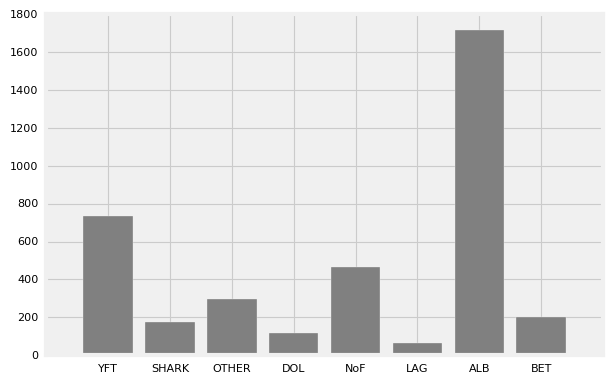
\includegraphics[width=\textwidth]{histogram_classes}
\end{figure}

Revisando el conjunto de datos encontramos varios problemas:

\begin{itemize}
\label{problems}
    \item{La distribución de imágenes entre las categorías es altamente desigual. La
categoría ALB tiene 1719 imágenes, que suponen más del 45 \% del conjunto
completo. Por otro lado, las dos categorías con menos ejemplos, DOL y LAG
contienen 117 y 67 imágenes respectivamente. Un modelo entrenado con este
conjunto de entrenamiento puede tener problemas clasificando estas categorías
con tan pocos ejemplos.}

\item{A la hora de dividir el conjunto en subconjuntos de entrenamiento, validación y
test hay que tener cuidado de dejar ejemplos de todas las categorías en cada
uno. Con tan pocos ejemplos es sencillo dejar una categoría completa fuera de un
conjunto al elegir imágenes aleatoriamente.}

\item{Si visualizamos las imágenes notamos que algunas son casi idénticas. Los
ejemplos de la figura \ref{same_image} parece que han sido sacadas de fotogramas
de un mismo vídeo. Esto reduce la diversidad de ejemplos que contienen cada
categoría. Teniendo una categoría con solo 67 ejemplos es preocupante que
algunos de las imágenes sean casi idénticas, ya que el modelo puede llegar a
usar características del barco en el que se encuentran los peces si mostramos
variaciones del mismo pez con el mismo fondo.}

\item{Se puede obsevar que en algunas imágenes los peces son muy difíciles de
        identificar, debido a que están parcialmente ocultos, la imagen está
        oscura o la cámara está sucia. Recordemos que algunas de las categorías
        son diferentes familias de atunes, con formas bastante parecidas.
    Distinguir entre dos familias de atunes en una imagen oscura y con el atún
parcialmente oculto puede llegar a ser imposible para un humano.}

\item{Algunas imágenes están mal etiquetadas. Si el modelo predice la clase
        incorrecta de la imagen (según su etiqueta) con mucha confianza, le
        asignará poca probabilidad a la clase correcta. Una probabilidad
        cercana a cero hará que la pérdida logarítmica aumente mucho.
}

\subsection{Conjuntos de test}

Para el envío de predicciones es necesario clasificar cada imagen del conjunto
de test que se proporciona en cada una de las fases de la competición. En la
primera fase el conjunto de test consta de 1000 imágenes para clasificar,
mientras que en la segunda consta de 13000.

No se ha realizado ningún tipo de inspección o exploración de ninguno de los
conjuntos de test para evitar cualquier tipo de sesgo a la hora de crear el
modelo. El segundo conjunto de test no se hizo público hasta seis días antes de
terminar la competición, por lo que era imposible saber qué tipo de imágenes
iba a contener. Una exploración del primer conjunto de test podría haber hecho
que se sobreajustara el modelo a este conjunto, empeorando la puntuación para
el siguiente conjunto si este era diferente.
        
\end{itemize}

\begin{figure}
  \caption{Dos imágenes del conjunto de entrenamiento casi idénticas}
\label{same_image}
  \makebox[\textwidth]{
  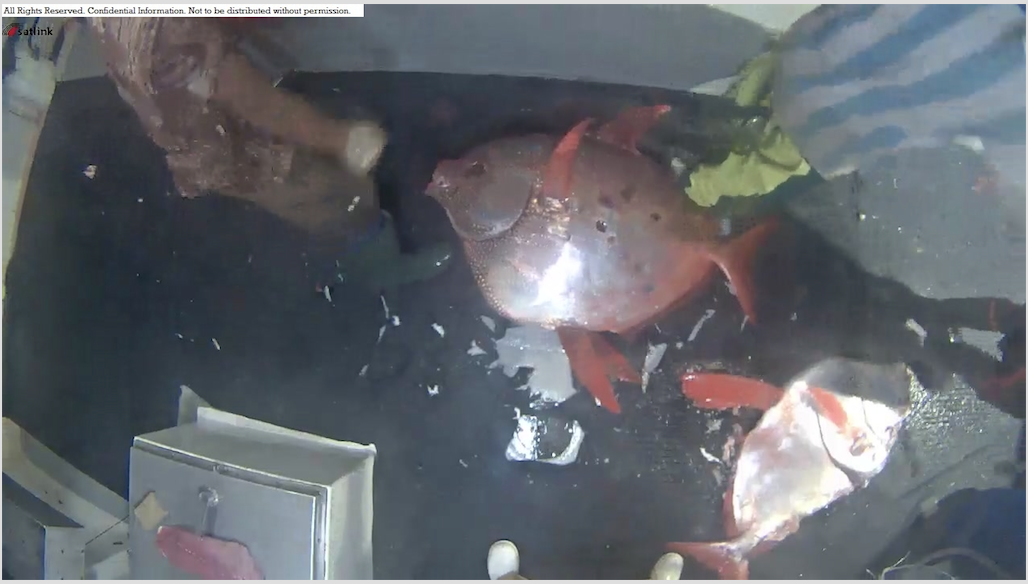
\includegraphics[width=0.4\linewidth]{fot1}
  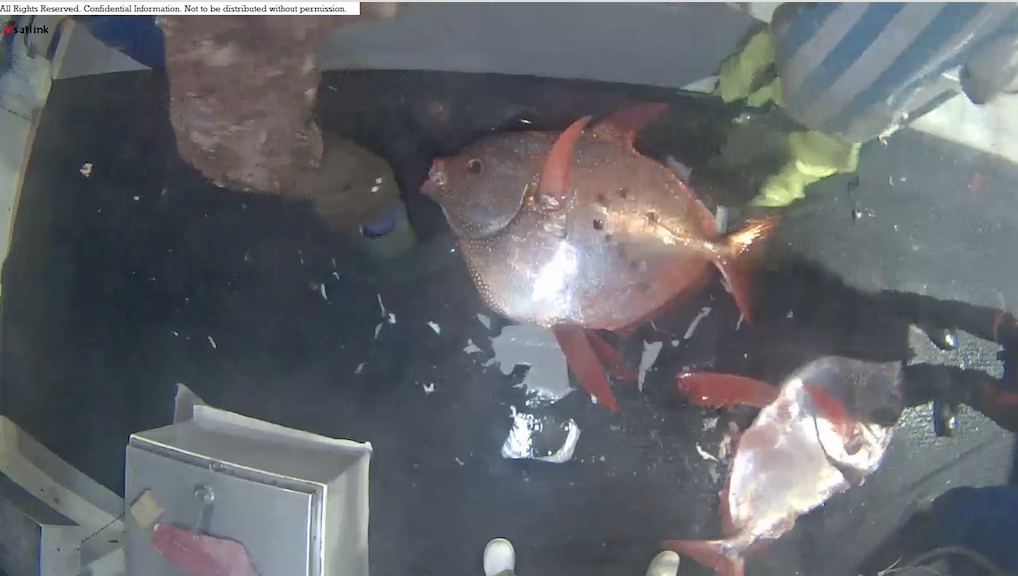
\includegraphics[width=0.4\linewidth]{fot2}
  }
\end{figure}
